\chapter{System do zarządzania wielokomputerowym serwerem WWW}
\label{r05}

\section{Wstęp}
W tym rozdziale zostanie przedstawiony opis konfiguracji stanowiska użytego do badań nad charakterystykami 
różnych konfiguracji i algorytmów klastra serwerów WWW zestawionego w środowisku systemu AIX i Windows NT z 
wykorzystaniem pakietu IBM WebSphere Performance Pack. Opisana zostanie konfiguracja sieci komputerowej, w której zostały 
przeprowadzone badania oraz charakterystyka poszczególnych testów.

\section{Charakterystyka użytego oprogramowania}

\subsection{IBM WebSphere Performance Pack}

IBM WebSphere Performance Pack jest oprogramowaniem infrastrukturalnym WWW wiążącym ze sobą skalowalność, niezawodność i 
wydajność, które to cechy są niezbędne dla aplikacji e-biznesu zarówno w środowiskach lokalnych jak i rozproszonych. Jego 
funkcje łączą ze sobą znakomity caching, zarządzanie plikami i równoważenie obciążenia, które razem kompensują wrodzone 
słabości Internetu by wspierać krytyczne aplikacje biznesowe.

IBM WebSphere Performance Pack składa się z trzech głównych elementów, które to pozwalają zredukować obciążenie serwera WWW, 
zwiększyć dyspozycyjność zasobów (zawartości) i zwiększyć wydajność serwera WWW \cite{GettingStarted}:
\begin{description}
\item[Współdzielenie plików]\

Komponent zajmujący się współdzieleniem plików, znany jako IBM AFS Enterprise File System (AFS), jest systemem plików 
pozwalającym współpracującym hostom (klientom i serwerom) efektywnie współdzielić zasoby systemów plików poprzez 
zarówno LAN jak i WAN. Prowadzi on replikację informacji pomiędzy wieloma serwerami w czasie rzeczywistym, gwarantując przy 
tym spójność danych, dostępność, stabilność i efektywność w administrowaniu, wymaganych przez duże, rozproszone serwisy webowe.
\item[Keszowanie i filtrowanie]\

Komponent odpowiedzialny za pamięć podręczną i filtrowanie zawartości webowej, znany jako IBM Web Traffic Express (WTE) jest 
proxy serwerem, który dostarcza wysoce skalowalnych funkcji keszowania i filtrowania związanych z przesyłaniem żądań webowych 
i dostarczaniem adresów URL. Moduł ten jest w stanie zredukować kosztowną szerokość wykorzystywanego pasma dostępowego i w 
szybszy sposób, oraz z mniejszymi opóźnieniami dostarczać informacje do klienta.
\item[Równoważnie obciążenia]\

Moduł odpowiedzialny za równoważenie obciążeń, znany jako IBM SecureWay Network Dispatcher jest serwerem zdolnym do 
dynamicznego monitorowania i równoważenia aplikacji i serwerów TCP w czasie rzeczywistym. Główną zaletą tego komponentu jest 
możliwość dynamicznego związania ze sobą wielu serwerów TCP tak, że wyglądają z sieci jak pojedynczy logicznie serwer.
\end{description}

Każdy z elementów IBM WebSphere Performance Pack może być zainstalowany oddzialenie od pozostałych -- także na innych 
komputerach. Dzięki związaniu tylu elementów w jednym pakiecie - klient otrzymuje oprogramowanie o scentralizowanej 
administracji i zminimalizowanym koszcie. 

Procedury instalacyjne pozwalają wybrać, który komponent należy zainstalować i na jakich maszynach w sieci mają się one 
znajdować. Oprogramowanie to jest portowane na następujące platformy: AIX (od wersji 4.2.1), Solaris (od wersji 2.6) oraz 
MS Windows NT i 2000.

\subsection{Web Traffic Express}
WTE jest naraz kaszującym serwerem proxy i filtrem zawartości pakietów. Zaawansowane keszowanie pozwala zminimalizować 
wykorzystanie przepustowości zwiększając przy tym pewność, że klienci spędzą znacznie mniej czasu podczas pobrania tej samej 
informacji kilka razy \cite{WTEUsersGuide,WTEProgramming}. 

Tradycyjny proxy serwer przesyła żądania dla URL od klienta i podaje je dalej do serwera przeznaczenia. WTE daje coś więcej; 
pozwala zapisać lub keszować dokumenty, które przesyła oraz serwować je podczas późniejszych żądań ze swojego keszu, a nie ze 
źródłowego serwera. Co oznacza, że klient żądany dokument otrzymuje szybciej przy zmniejszonym obciążeniu łącz. 

Moduł ten posiada także dodatkowe cechy takie jak:
\begin{itemize}
\item możliwość utrzymania bardzo dużego keszu;
\item opcję automatycznego odświeżania tej części pamięci podręcznej zawierającej najczęściej popobierane strony;
\item możliwość keszowania także tych stron, których nagłówek wymaga by były zawsze pobierane ze źródłowego serwera;
\item konfigurowania okresowego porządkowania keszu z informacji bezużytecznych w celu poprawy wydajności i utrzymania 
efektywności jego działania;
\item Remote Cache Access (RCA) - właściwość pozwalająca na wielu maszynom z WTE uwspólniania tego samego keszu poprzez 
rozproszony system plików, taki jak AFS, w celu zredukowania redundancji zawartości.
\end{itemize}

Dodatkowo WTE pozwala na ustawianie filtrowania zawartości na poziomie serwera proxy -- pozwalając na takie zabiegi jak np. 
blokowanie URL--ów. Zwielokrotnione serwery WTE mogą być obciążeniowo zrównoważone.

Kolejną cechą jaką posiada ten moduł jest możliwość pracy jako przezroczysty proxy -- czyli taki, do którego działania nie jest 
potrzebna żadna zmiana w konfiguracji przeglądarki klienta -- WTE pracuje wtedy na porcie serwera WWW. 

\subsection{IBM SecureWay Network Dispatcher}
Jest to jedno z pierwszych komercyjnych rozwiązań, które pozwala zwiększyć wydajność i zapewnić ciągłą pracę serwisów 
internetowych. Znalazło ono już szerokie zastosowanie w znaczących serwisach WWW, takich jak serwisy prowadzone w trakcie 
olimpiad w Atlancie i Nagano. 
System jest przeznaczony do obsługi serwerów webowych zbudowanych w technologii klastrowej. Klaster jest grupą serwerów 
webowych obsługujących jedną witrynę WWW. Wszystkie serwery w klastrze posiadają tę samą zawartość i zapytanie może być 
obsłużone przez dowolny z nich serwer. Pojedyncze zapytanie obsługiwane jest przez jeden z aktualnie sprawnych serwerów. 
IBM SecureWay Network Dispatcher składa się z trzech komponentów: podsystemu Dispatcher, podsystemu Interactive Session 
Support (ISS) oraz podsystemu Content--based Routing (CBR). Komponenty te mogą być używane łącznie lub każdy z 
osobna \cite{LoadBalancingWithND}.

\subsubsection{Komponent Dispatcher}

Podstawowym komponentem systemu jest Dispatcher, którego zadaniem jest zapewnienie równomiernej dystrybucji zapytań 
realizowanych za pośrednictwem protokołu TCP/IP między wieloma serwerami realizującymi tę samą usługę w konfiguracji 
klastrowej. Funkcjonowanie Network Dispatcher'a opiera się na architekturze przedstawionego wcześniej dystrybutora. 
Dispatcher może równoważyć obciążenia w obrębie sieci lokalnej lub rozległej. Dla każdego klastra definiuje się porty, które 
chcemy, aby były obsługiwane przez klaster, następnie serwery, które będą dostarczać usługi na każdym z zdefiniowanych portów. 
Dispatcher może obsługiwać wiele klastrów \cite{NDUsersGuide}. 

Wysoką dostępność serwisu osiągnięto poprzez działanie samego Dispatcher'a, który wykrywa niesprawne serwery w klastrze i 
omija je przy dystrybucji zapytań oraz poprzez wprowadzenie drugiego systemu Dispatcher'a. W podstawowym trybie pracy 
Dispatcher wymaga, aby wszystkie serwery w klastrze były w tej samej podsieci co Dispatcher. Wówczas, aby podwyższyć 
dostępność serwisu, możemy skonfigurować drugi system Dispatcher'a, który pełnić będzie rolę maszyny zapasowej i czuwającej w 
gotowości do przejęcia zadania równoważenia obciążenia w przypadku, gdyby maszyna podstawowa Dispatcher'a przestała działać 
poprawnie. Mechanizm typu heartbeat zapewnia monitorowanie stanów przez obie maszyny, podstawową i zapasową oraz przejęcie 
zadań w przypadku wystąpienia awarii.
\begin{figure}[h]
\centering
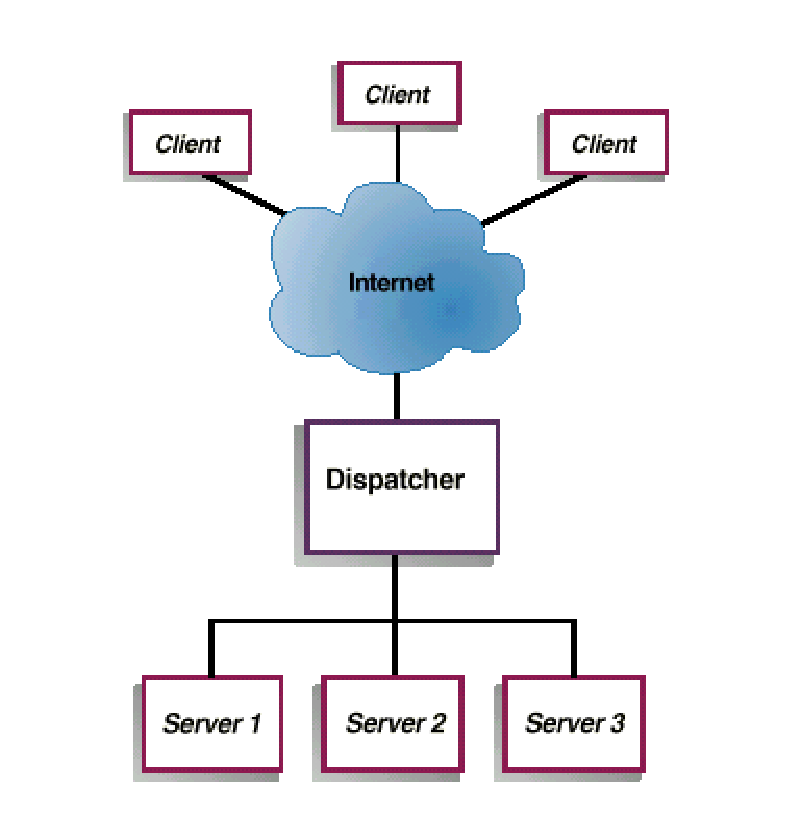
\includegraphics[width=3in]{./rysunki/dispatcher.eps}
\caption{Konfiguracja logiczna modułu dispatcher}
\label{dispatcher}
\end{figure}

Dispatcher realizuje swoje zadania za pomocą trzech wewnętrznych komponentów: Egzekutora, Menadżera i Doradców. Egzekutor 
realizuje równoważenie obciążeń. Dla pakietu wysyłanego w ramach nowego połączenia między klientem a serwerem WEB Dispatcher 
sprawdza, który z serwerów może przejąć obsługę zlecenia na żądanym przez klienta porcie i adresie klastra. Następnie, dla 
każdego takiego serwera, na podstawie zgromadzonych wag określających poziom obciążeń serwerów, określa serwer najmniej 
obciążony, do którego przekazuje pakiet. Jeśli połączenie już istnieje, wtedy bez żadnego przetwarzania pakiet jest natychmiast
wysyłany do tego samego serwera, który został wybrany podczas inicjalizacji połączenia. Rozdział zleceń między serwery bazuje 
na wartościach wag wskazujących na możliwość potencjalnego obciążenia serwera -- np. jeżeli jeden serwer ma wagę 2, a drugi ma 
wagę 1, to serwer o wadze 2 powinien dostać dwa razy więcej żądań niż ten o wadze 1. Wagi mogą być ustawiane ręcznie lub przez 
Menadżera. Najczęściej do ustawiania wag korzysta się z Menadżera, który ustawia wagi automatycznie i w sposób adaptacyjny, z 
uwzględnieniem aktualnych warunków pracy klastra. Menadżer może korzystać z wewnętrznych liczników systemowych oraz z 
informacji dostarczanych przez inne komponenty systemu, takich jak ISS czy WLM. Zarządca decyduje który z serwerów jest 
najmniej obciążonym poprzez obserwację wag serwerów, które to okresowo analizuje i uaktualnia. Decyzję jaką serwerowi nadać 
wagę podejmuje opierając się na czterech parametrach:
\begin{itemize}
\item liczba aktywnych połączeń realizowanych na każdym serwerze TCP;
\item liczba nowych połączeń na każdym serwerze TCP;
\item danych wejściowych pochodzących od doradców;
\item informacji pochodzących od narzędzi monitorujących pracę systemu, takich jak ISS;
\end{itemize}

Używanie zarządcy jest opcjonalne, ale jeśli 
nie jest on używany, równoważenie obciążenia jest dokonywane przy użyciu marszrutowania algorytmem ważonego Round Robina, 
gdzie wagi poszczególnych serwerów WWW są nadawane statycznie; 

Aby dać administratorowi większą kontrolę nad tym, gdzie kierowane będą żądania różnego typu pochodzące od różnych grup 
użytkowników, wprowadzono pojęcie reguł i grup serwerów im podległych, tj. serwerów, wśród których będzie realizowane 
równoważenie obciążenia w razie spełnienia reguły. Dla Dispatcher'a dostępne są reguły bazujące na: adresie IP klienta, porcie 
klienta, porze dnia, połączeniach na sekundę dla danego portu, aktywnych połączeniach dla danego portu. Reguły dają możliwość 
implementacji wysokiej jakości usług dla wybranych klientów bądź w określonej porze dnia. Dostępna jest także reguła ,,zawsze 
prawdziwe'', która oznacza spełnienie zadanego warunku dla wszystkich przyjmowanych zleceń.
\begin{figure}[h]
\centering
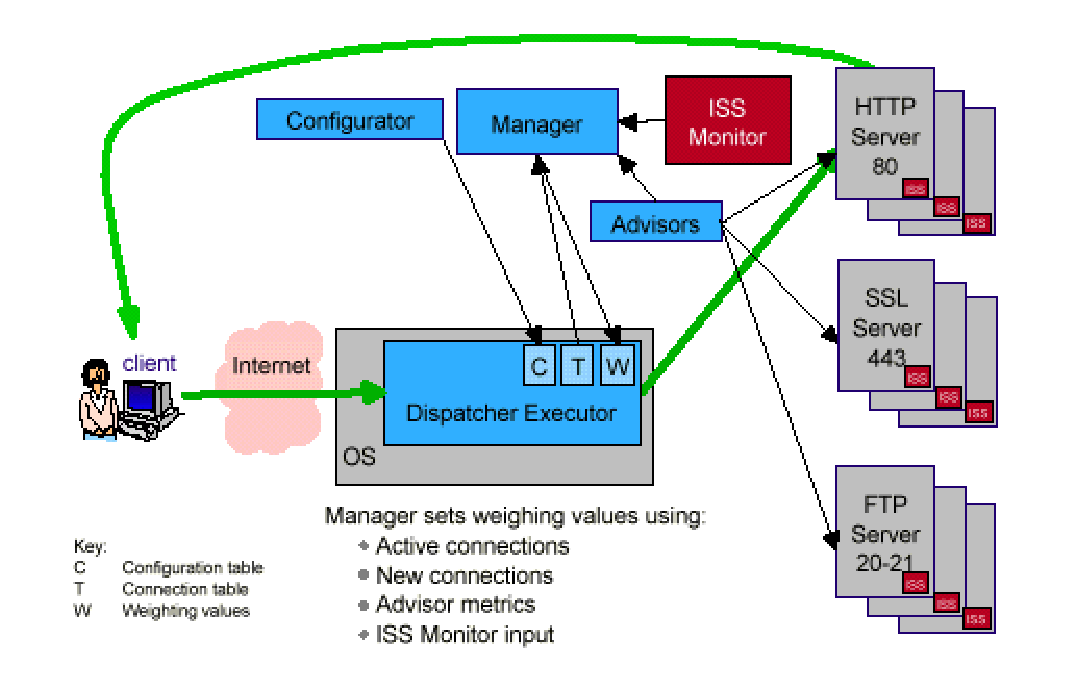
\includegraphics[width=5in]{./rysunki/executor.eps}
\caption{Architektura Network Dispatcher-a}
\label{dispatcher1}
\end{figure}

Zadaniem doradców jest zbieranie informacji na temat obciążenia serwerów. Doradcy sprawdzają również, czy serwery, na których 
dokonywane jest równoważenie obciążeń, funkcjonują prawidłowo. Doradcy okresowo otwierają połączenia TCP i wysyłają do serwera 
wiadomość z żądaniem specyficznym dla danego typu doradcy. Po wysłaniu wiadomości Doradcy czekają na odpowiedź. Po jej 
otrzymaniu większość Doradców szacuje wartość obciążenia serwera na podstawie czasu, jaki upłynął nim serwer zwrócił odpowiedź 
na żądanie i zgłaszają ten czas (w milisekundach) Menadżerowi, aby ten na podstawie tej i innych informacji oszacował wartość 
wag poszczególnych serwerów. 

Wraz z produktem IBM SecureWay Network Dispatcher dostarczeni są doradcy: HTTP, FTP, Telnet, NNTP, POP3, SMTP, SSL, WTE, TCP, 
Ping, WLM. Istnieje również możliwość napisania własnego doradcy. 

\subsubsection{Komponent Interactive Session Support}

Interactive Session Support (ISS) jest komponentem współpracującym z Domain Name Server (DNS) w jednym z trzech możliwych 
trybów pracy: DNS--Update, DNS--Replace lub DNS--Ignore. Komponent ten może być również wykorzystany do zbierania informacji na 
temat obciążenia serwerów, którą następnie przekazuje do Dispatcher'a. W trybie DNS--Update ISS uaktualnia serwer nazw DNS. W 
tym trybie działa on w połączeniu z serwerem nazw w celu mapowania nazw DNS na adresy IP serwerów najlepiej nadających się do 
obsługi danego zadania. W trybie DNS--Replace ISS spełnia dla ograniczonej podgrupy sieci funkcję serwera nazw, nie zawiera 
jednak wszystkich funkcji standardowego DNS. W trybie DNS--Ignore, ISS działa w połączeniu z Dispatcher'em w celu lepszego 
równoważenia obciążeń.
\begin{figure}[h]
\centering
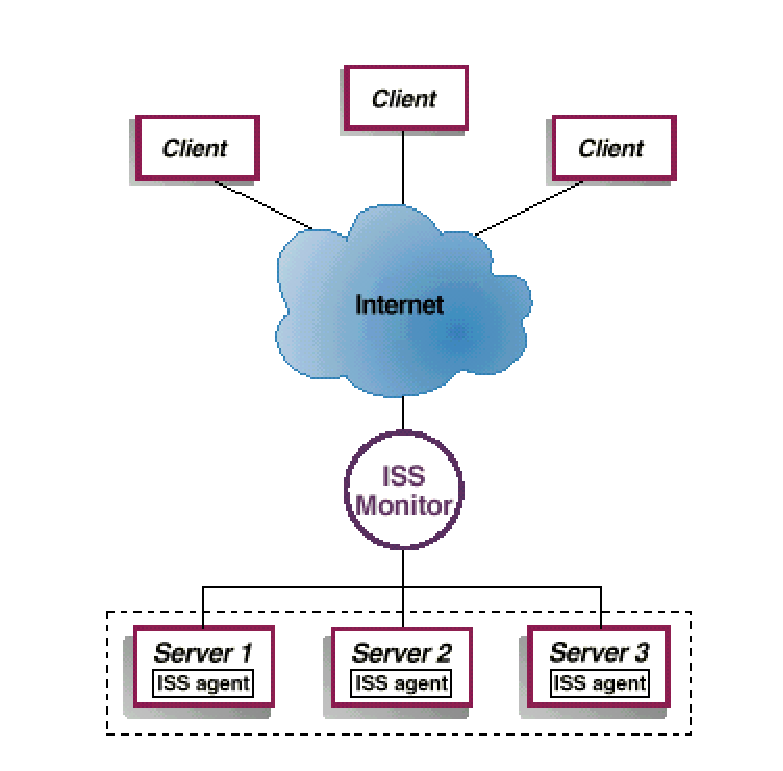
\includegraphics[width=3in]{./rysunki/ISS.eps}
\caption{Konfiguracja logiczna modułu Interactive Session Support}
\label{ISS}
\end{figure}

Obciążenie na poszczególnych węzłach może być określane poprzez pomiar wykorzystania różnych zasobów, takich jak ilość wolnej 
pamięci, użycie procesora czy licznik procesów. ISS posługuje się jedną z trzech strategii alokacji zleceń: RoundRobin, Best, 
i Statistical RoundRobin.

Przy użyciu algorytmu RoundRobin, ISS równoważy obciążenia serwerów w sposób klasyczny dla tej strategii. Z danej grupy 
serwerów ISS wybiera na określony przedział czasu jeden serwer, który będzie obciążany w tym przedziale czasu. ISS nie zwraca 
wówczas uwagi na poziom obciążenia serwera, ale też nie zaleci serwera, który niedomaga. Takie podejście może funkcjonować 
dobrze, pod warunkiem że obciążenie wywoływane przez klientów jest równomierne. Zaletą tej metody jest brak obciążenia 
serwerów poprzez procesy pomiarowe. Natomiast jej dużą wadą jest brak elastyczności. Metoda ta może powodować, że np. serwer, 
który już jest bardzo obciążony, może być dalej preferowany przez ISS, gdyż nie skończył się jeszcze przydzielony mu czas.
Stosując strategię Best, w czasie trwania określonego interwału, ISS trasuje żądania do serwera, który na początku tego 
interwału miał najniższy poziom obciążenia. Tak jak w przypadku poprzedniej metody, korzystający z niej ISS nie zaleci 
serwera, który przestał funkcjonować. Ta metoda selekcji sprawdza się bardzo dobrze dla każdego czasu trwania połączeń, pod 
warunkiem, że częstość nowych połączeń będzie relatywnie niska w stosunku do ustawionego interwału czasu przydziału dla 
pojedynczego serwera. Ta strategia jest przyjmowana domyślnie przez system.
W strategii Statistical RoundRobin, ISS równoważy obciążenia na podstawie statystyk obciążenia, które generuje dla wszystkich 
serwerów. Wykorzystuje te statystyki do budowy profilu najbardziej i najmniej obciążonych serwerów, a następnie w ciągu 
trwania interwału ,,heartbeat'' rozdziela żądania pomiędzy serwery, proporcjonalnie do ich obciążenia. Również przy użyciu tej 
metody ISS nie zaleci niedomagającego serwera. Metoda ta sprawdza się wszędzie tam, gdzie występuje duża częstość 
krótkotrwałych połączeń.

\subsubsection{Komponent Content Base Routing}
 
Komponent CBR może być skonfigurowany z WTE (Web Traffic Express) dla serwerów HTTP, lub jako CBR proxy (bez współpracy z WTE)
dla serwerów IMAP i POP3. CBR współpracuje wespół z Web Traffic Express, w ten sposób, że klient wysyła żądanie do WTE, który 
jest skonfigurowany by móc korzystać z CBR; CBR musi być zainstalowany na tej samej maszynie co serwer WTE. WTE wypytuje 
komponent CBR który serwer ma obsłużyć żądanie. Gdy CBR otrzyma żądanie próbuje je dopasować do ustawionych reguł. Jeśli 
pasują, CBR wybiera serwer, z grupy skonfigurowanych do odbierania konkretnego typu żądań, jednocześnie równoważąc pomiędzy 
tą grupą serwerów obciążenie. 

CBR jest bardzo podobny w strukturze do pakietu Dispatcher. Trzy kluczowe elementy CBR (Egzekutor, Menadżer i Doradcy) 
współpracują by zrównoważyć i rozdzielić przychodzące żądania pomiędzy serwery w zbliżony sposób jak w Dispatcherze. 
Jednakże w przeciwieństwie do modułu Dispatcher -- CBR nie oferuje funkcji zwiększonej dostępności. Jednakże można połączyć 
kilka serwerów CBR i równoważyć ich obciążenie poprzez serwer ND, który to może sprawdzać czy żaden z CBR serwerów nie 
przestał odpowiadać.

\begin{itemize}
\item CBR z WTE (obsługujący ruch HTTP)

Komponent CBR współpracując z Web Traffic Express działa jako proxy serwer przekierowując rządania klientów do odpowiednich
serwerów. Moduł WTE jest proxy serwerem, pozwalającym manipulować pamięcią podręczną w celu szybkiego transferu dokumentów
przy niewielkich wymaganiach dotyczących przepustowości sieci. CBR zaś jest w stanie przefiltrować zawartość stron WWW 
korzystając ze specyficznych ciągów warunków nazywanych rolami. CBR daje możliwość określenia grupy serwerów, które powinny
przejąć żądanie opierając się na wyrażeniach regularnych pasujących do zawartości żądania. Ponieważ CBR pozwala na
,,przywiązanie'' poszczególnych serwerów do każdego typu żądania następuje zrównoważenie obciążenia serwerów. CBR potrafi
także wykrywać kiedy serwer przestaje odpowiadać wyłączając routing żądań do niego. Zastosowane w module CBR algorytmy
równoważenia obciążenia są identyczny z tymi zastosowanymi w komponencie Dispatcher. 

Sposób działania CBR: gdy klienckie żądanie jest przesyłane do WTE proxy następuje tu korelowanie zawartości żądania
z regułami zdefiniowanymi w module CBR. Jeśli zbiór reguł pasuje do zawartości żądania jeden z serwerów ,,związanych'' z 
obsługą tego typu żądań zostaje wybrany do przyjęcia żądania. Wtedy WTE jako proxy serwer przekierowuje do wybranego serwera 
żądanie. Jak widać moduł WTE musi być uruchomiony zanim CBR zostanie skonfigurowany, ponieważ działa on jako podproces WTE.
Oczywiście oba moduły muszą znajdować się na tej samej maszynie.

Oznacza to podział farmy serwerów na części realizujące odpowiedni typ żądań. Taki podział jest przezroczysty dla klienta. 
Można np. podzielić witrynę na dwie części -- kilka serwerów realizujących tylko żądania CGI, a pozostałe resztę ruchu HTTP.
Pozwala to na realizację intensywnie przetwarzanych skryptów CGI w sposób nie kolidujący z pracą reszty serwerów WWW 
obsługujących normalny ruch HTTP -- co oznacza dla klienta lepszy ogólny czas odpowiedzi. W ten sposób komputery o większej
mocy obliczeniowej można przeznaczyć na obsługe normalnego ruchu bez kosztownego upgradu wszystkich komputerów.
\begin{figure}[h]
\centering
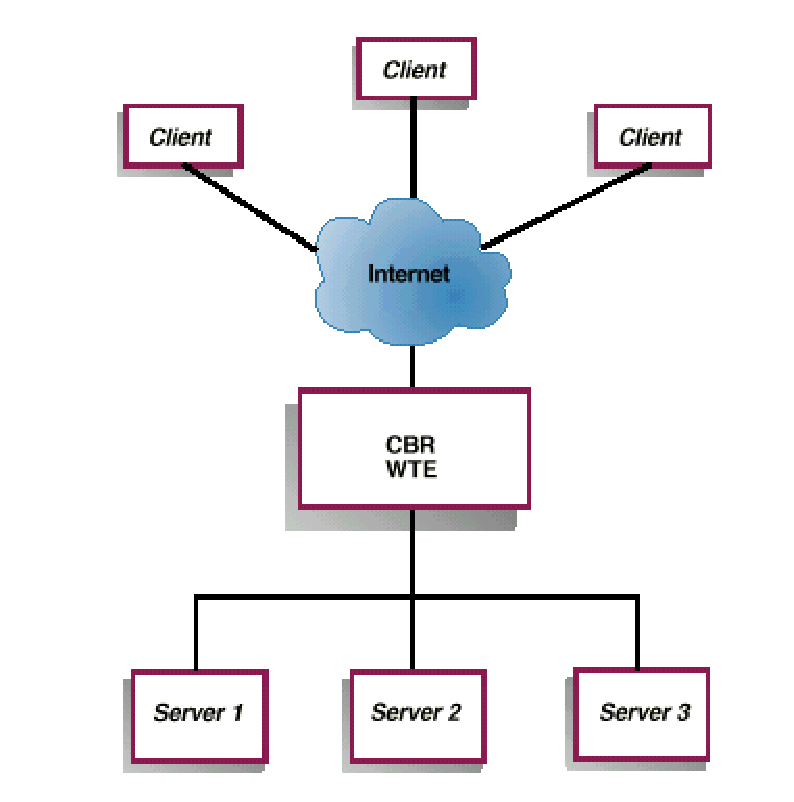
\includegraphics[width=3in]{./rysunki/CBR-WTE.eps}
\caption{Konfiguracja logiczna modułu Content Base Routing (wraz z WTE)}
\label{CBR}
\end{figure}


Inną możliwością podziału serwera WWW jest bezpośrednie przekierowanie klientów, którzy chcą dostać się do stron wymagających
rejestracji, do jednego typu serwerów, a resztę do pozostałych. Wtedy obsługą stron wymagających rejestracji zajmują się
np. komputery o większej mocy obliczeniowej i klienci, którzy są już zarejestrowani mają lepszy czas odpowiedzi niż inni. 

Wybierając role dokonujące równoważenia obciążenia należy sprawdzić czy wszystkie żądania do klastra WWW posiadają role, 
na podstawie ktorych można wybrać serwer. Jeśli tak nie jest, tzn. jeśli przychodzące żądanie nie pasuje do żadnej roli, klient
otrzyma komunikat o błędzie pochodzący z WTE. Najprostszym rozwiązaniem jest stworzenie roli zawsze prawdziwej z bardzo 
wysokim priorytetem i ,,przywiązanie'' jej do osobnej grupy serwerów.

\item CBR proxy (obsługujący ruch IMAP i POP3)

CBR bez WTE może być proxy wybierającym odpowiedni serwer opierając się na ID użytkownika i haśle. Nie wspiera wtedy opartego
na rolach równoważenia obciążeń.
\end{itemize}

\subsection{Content Base Routing -- konfiguracja}

CBR może zostać skonfigurowany jako proxy dla usług opartych o protokoły POP3 lub IMAP -- działa wtedy bez współpracy
z modułem WTE, lub tez jako narzędzie równoważące obciążenie ruchu HTTP -- systemem proxy jest wtedy WTE  \cite{NDUsersGuide}.

Moduł ten można skonfigurować za pomocą linii komend lub z pomocą graficznego interfejsu użytkownika
(\emph{GUI}). Moduł Content Base Routing jest bardzo podobny w architekturze do Dispatchera. Składa się on z trzech
funkcjonalnych części:
    \begin{itemize}
    \item Egzekutor -- zajmuje się równoważeniem obciążenia zapytań klienckich. Jest zawsze uruchomiany jeśli CBR
    jest w użyciu;
    \item Menadżer -- ustala wagi dla poszczególnych serwerów opierając się na:
        \begin{itemize}
        \item wewnętrznych licznikach Egzekutora;
        \item informacjach zbieranych z serwerów przez doradców;
        \item informacjach z programów monitorujących prace systemu, takich jak ISS czy WLM.
        \end{itemize}
        Korzystanie z menadżera jest opcjonalne. Jednakże gdy jest on nieużywany -- równoważenie obciążenia jest
        realizowane za pomocą algorytmu statycznego Ważonego Round--Robin opartego na domyślnych wagach, a
        doradcy nie będą wtedy dostępni.
    \item Doradcy -- wypytują serwery oraz analizują dane o ich stanie, by następnie z tak spreparowanych danych
    Menadżer ustalił odpowiednie wagi. Korzystanie z Doradców jest również opcjonalne, a typowej konfiguracji wręcz
    może nie być potrzebne, jednakże mimo to poleca się z nich korzystać.
    \end{itemize}

Wszystkie trzy części (Egzekutor, Menadżer oraz Doradcy) współpracują ze sobą w celu rozbalansowania i
rozpropagowania przychodzących żądań pomiędzy serwery.

Aby skonfigurować wstępnie CBR, można posłużyć się jedna z czterech dostępnych metod:
    \begin{enumerate}
    \item Linii komend;
    \item Skryptów konfiguracyjnych;
    \item Graficznego interfejsu użytkownika;
    \item Konfiguracyjnego wizarda.
    \end{enumerate}

\subsubsection{Konfiguracja maszyny CBR}

Aby moc konfigurować CBR, należy mieć status root--a w systemie. Należy także znać adresy każdego z
konfigurowanych klastrow serwerów. Pojedynczy adres IP jest tu używany jako jeden adres dla całego klastra.
Zanim jednakże przeprowadzi się konfiguracje i uruchomienie modułu CBR -- musi być już skonfigurowany i
uruchomiony WTE. Konfiguracje wykonuje się w takiej kolejności (konfiguracja dotyczy tylko ruchu HTTP):
    \begin{enumerate}
    \item Uruchomienie WTE
    \item Po uruchomieniu WTE, należy zdefiniować klaster WWW, oraz ustawić specyficzne dla tego
    klastra opcje. Do zdefiniowania klastra oraz opcji służy komenda:\\
    
    cbrcontrol cluster set \emph{cluster opcja wartość}\\
    
    \item Następnym krokiem jest zdefiniowanie portów ustalenie ich opcji. Wykonuje się to komendą:\\
    
    cbrcontrol port set \emph{cluster:port opcja wartość}\\
    
    \item Definiowanie poszczególnych komputerów należących do serwera:\\
    
    cbrcontrol server add \emph{cluster:port:server}\\
    
    gdzie \emph{server} jest nazwą symboliczną pojedynczego komputera w klastrze, lub jego adresem IP;
    \item Następnym krokiem jest konfiguracja reguł CBR. Jest to krok kluczowy w konfiguracji CBR przy ruchu po protokole HTTP
    reguły (role) definiują jak zadanie URL zostanie przesłane do jednego lub większej ilości serwerów. Te specyficzne
    reguły nazywają się regułami zawartosci\footnote{\emph{and. -- content rule}}. Aby zdefiniować regułę
    korzysta się z następującej komendy:\\
    
    cbrcontrol rule add \emph{cluster:port:rule} type content pattern=\emph{pattern}\\
    
    gdzie wartość \emph{pattern} jest wyrażeniem regularnym, które będzie porównywane za każdym razem jak
    nadejdzie żądanie od klienta.
    \item Następnie należy dodać poszczególne serwery obsługujące reguły zawartości. Gdy występuje dopasowanie
    pomiędzy żądanym URL, a regułą zawartości zostaje wybrany najlepszy z serwerów obsługujących ten typ
    żądań. Aby wykonać takie dopasowanie -- reguła dopasowania--serwer obsługujący wykonuje się polecenie:\\
    
    cbrcontrol rule useserver \emph{cluster:port:rule server}\\
    
    \item Uruchomienie Menadżera (opcjonalne):\\
    
    cbrcontrol manager start\\

    \item Uruchomienie Doradców (opcjonalne):\\

    cbrcontrol advisor start http \emph{port}

    \item Ostatnim krokiem jest skonfigurowanie Doradców, aby ich informacje brały udział w decyzjach równoważenia
    obciążenia.
    
    \end{enumerate}

\subsubsection{Konfiguracja LB opartego na regułach}

Wykorzystując do równoważenia obciążenia WTE wraz z modułem CBR -- można rozdzielać ruch sieciowy
wykorzystując następujące typy reguł:
    \begin{itemize}
    \item Adres IP klienta; jest to sytuacja, gdy wymaga się alokacji zasobów w zależności od tego skąd przychodzi
    zadanie. Można założyć, ze z pewnych adresów (od klientów) wymagamy by zadania nie były realizowane, zatem
    przygotowuje się regule i nie dodaje do żadnego serwera -- wtedy określeni klienci nie będą obsługiwani
    (wystąpi błąd). np.:\\

    ndcontrol rule add 9.67.131.153:80:ni type ip beginrange 9.0.0.0 endrange \
    9.255.255.255\\

    taka reguła oznacza, ze klienci z domeny IBM--a nie osiągną serwera CBR;        
    \item Godzina połączenia; taką regułę wykorzystuje się głownie przy określonych planach obsługi obciążeń.
    W przypadku gdy witryna produkcyjna otrzymuje pewna grupę żądań o pewne dokumenty w określonym
    (i stałym) czasie każdego dnia -- można tylko dla tych żądań wyznaczyć osobne serwery; może to być także
    przydatne w przypadku gdy w godzinach nocnych (najmniejszy ruch) -- niektóre maszyny z powodu wykonywania
    backupu powinny być wyłączone z realizacji żądań;
    \item Ilość połączeń na sekundę, na port; (działa tylko podczas uruchomionego Menadżera) można wykorzystywać
    np. w przypadku: \emph{if połączeń na sekundę na porcie 80 > 100 then użyj te dwa serwery}, \emph{if połączeń
    na sekundę na porcie 80 > 2000 użyj te 8 serwerów};
    \item Całkowita ilość aktywnych połączeń na porcie; (wymóg jak wyżej -- Menadżer musi być uruchomiony);
    Jest to reguła potrzebna w przypadku gdy wiadomo kiedy serwer będzie np. przeładowany (przy ilu połączeniach)
    Jeśli np. wiadomo, ze serwer nie jest w stanie przyjąć i zrealizować naraz więcej niz. 250 jednoczesnych połączeń
    tworzy się regułę:\\

    ndcontrol rule add 130.40.52.153:80:pool2 type active beginrange 250 endrange 500\\

    Wtedy do tak stworzonej reguły do pojedynczego serwera można dodać następne maszyny, które w przypadku
    większej ilości połączeń zostaną włączone w podejmowanie żądań;
    \item reguła zawsze prawdziwe; Reguła ta jest zawsze spełniona -- chyba ze serwery z którymi jest związana
    nie pracują; przydają się w przypadku gdy nie chcemy aby jakikolwiek klient dostał zwrot w postaci błędu
    zadania dokumentu (od WTE);
    \item Zawartość zadania; (jest to reguła dostępna tylko z poziomy modułu CBR); reguła wykorzystywana
    w przypadku dystrybucji żądań w zależności od zawartości zadania; np. gdy potrzeba aby jedna grupa serwerów
    obsługiwała zadania \emph{cgi--bin}, inna grupa obsługiwała media strumieniowe (np. real media), zaś trzecia wszystkie
    pozostałe wtedy wzorcem pierwszej z reguł 
    będzie ścieżka do katalogu cgi--bin, drugiej do plików strumieniowych, a trzeciej reguła zawsze prawdziwe;
    następnie należy tylko przyporządkować reguły do odpowiadających im grup serwerów;
        \begin{description}
        \item[Typy reguł dla CBR]\

        składnia wzorców reguł wygląda następująco: w regule (wzorcu)  nie może być żadnych przerw (spacji)
        ani znaków specjalnych:
            \begin{description}
            \item[*] -- odpowiada 0 do x wystąpienia dowolnych znaków;
            \item[)(] -- używane do grupowania logicznego;
            \item[\&] -- logiczne AND;
            \item[|] -- logiczne OR;
            \item[!] -- logiczne NOT;
            \end{description}
        Zarezerwowane słowa (zawsze następuje do nich przyporządkowanie w postaci znaku równości):
            \begin{description}
            \item[client] -- adres IP klienta;
            \item[url] -- URL w zadaniu;
            \item[path] -- sekcja ścieżka URL--a;
            \item[protocol] -- sekcja protokółu URL--a;
            \item[refer] -- \emph{quality of service}
            \end{description}
        Poniżej znajdują się przykłady:\\

        \emph{url=http://*/*.gif}\\

        \emph{client=9.32.*}\\

        \emph{!(path=*.jpeg)}\\

        \emph{(path=index/*.gif \& protocol=httpd) | (client=9.1.2.3)}       
        \end{description}
    \end{itemize}

Wszystkie reguły posiadają nazwę, typ, priorytet, początkowy zakres działania, końcowy zakres działania oraz
grupę obsługujących serwerów. Dodatkowo, reguła zawartości w komponencie CBR posiada związane ze sobą
wyrażenie regularne. Reguły są wykorzystywane w kolejności ich priorytetów. Reguły z niskim priorytetem są
realizowane wcześniej. Innymi słowy, reguła z priorytetem 1 jest wykorzystywana przed reguła o priorytecie 2.
Pierwsza poprawnie dopasowana reguła zostaje wykorzystana (reszta już nie jest próbkowana).

Aby reguła została spełniona musza być spełnione naraz dwa warunki:
    \begin{enumerate}
    \item Predykat reguły musi być prawdziwy. Co oznacza, ze wartość porównana musi znajdować się pomiędzy
    wartościami początkowa i końcowa, lub zawartość zadania musi pasować do wyrażenia regularnego
    wyspecyfikowanego w wzorcu\footnote{ang. \emph{pattern}}. Dla reguł o typie ,,zawsze prawdziwy''
    reguła jest zawsze spełniona (bez warunków);
    \item Jeśli istnieją serwery związane do poszczególnych reguł, co najmniej jeden z nich musi być dostępny do
    odebranie zadania.
    \end{enumerate}

W przypadku, gdy nie ma serwerów dla których konkretna reguła nie mogłaby być spełniona -- zadanie zostaje
porzucone, a CBR zwróci do serwera proxy (WTE) komunikat błędu. Jeśli zaś żadna z reguł nie może zostać
spełniona -- jak wyżej -- CBR zwróci do WTE komunikat błędu.

\subsection{Narzędzie do testów -- Astra Load Runner}

Narzędziem testowym w wykonanym projekcie było oprogramowanie firmy Mercury Interactive\footnote{http://www.merc-int.com}
-- Astra Load Runner. Jego wybór był spowodowany szerokim wachlarzem możliwości testowych, obsługiwanych protokołów oraz
możliwości dokonywania analiz i wizualizacji rezultatów. Poniżej znajduje się krótka charakterystyka tego progrmau:

LoadRunner jest narzędziem do testów wydajnościowych, dzięki którym można sprawdzić wydajność i skalowalność systemu webowego.
Jest on w stanie generować dziesiątki, setki czy nawet tysiące jednoczesnych użytkowników, umożliwiając w ten sposób wykrycie 
wszystkich słabych, bądź niewydajnych miejsc w naszym systemie. W czasie trwania testu dostępne są różnorakie 
monitory, wyświetlające cały czas wszystkie interesujące parametry systemu funkcjonującego pod obciążeniem. Dzięki 
tym wbudowanym monitorom można np.:  na bieżąco śledzić czasy odpowiedzi wszystkich serwerów, czasy wykonywania się danych 
transakcji czy szybkość transferu danych w sieci z podziałem na segmenty.

Wszyscy użytkownicy generowani przez LoadRunnera kontrolowani są z jednego centralnego modułu zwanego kontrolerem. Testując 
system pod obciążeniem można symulować różne numery IP klientów, różne przeglądarki internetowe oraz różne 
szybkości łączy internetowych, cały czas jednocześnie monitorując zachowanie naszego obciążanego systemu.
Dane Techniczne Narzędzia:
\begin{description}
\item[Wspierane protokoły typu klient/serwer]\
	\begin{itemize}
	\item Oracle UPI
	\item Oracle OCI
	\item ODBC
	\item MS-SQL Server
	\item Sybase ctlib
	\item Sybase dblib
	\item Informix I-Net
	\item DB2 CLI
	\item Tuxedo (including compression mode)
	\item RTE
	\item CORBA
	\item COM/DCOM
	\item WinSocket
	\end{itemize}
\item[Wspierane protokoły ERP]\
	\begin{itemize}
	\item SAP R/3
	\item PeopleSoft (2-tier i Tuxedo-based)
	\item Oracle Applications
	\item Siebel
	\item Baan
	\end{itemize}
\item[Wspierane protokoły internetowe]\
	\begin{itemize}
	\item Streaming (Real Audio and Real Video)
	\item MS Media
	\item iMode
	\item VoiceXML
	\item LDAP
	\item WAP--HTTP
	\item WAP--Gateway
	\item HTTP
	\item HTTPS (SSL)
	\item Digital Certificates
	\item RMI
	\item FTP
	\item POP3
	\item Winsock
	\item SMTP
	\end{itemize}
\item[Wspierane systemy Legacy]\
	\begin{itemize}
	\item 3270 Terminals (Mainframe)
	\item 5250 Terminals (AS/400)
	\item VT    Terminal   (DEC)
	\item X Window Applications
	\end{itemize}
\item[Tworzenie testów wydajnościowych:]\
	\begin{itemize}
	\item Możliwość przełączania rodzaju nagrywanego protokołu w trakcie rejestracji jednego skryptu;
	\item Narzędzie automatycznie generuje skrypty testów obciążeniowych, oparte na operacjach biznesowych wykonywanych na 
	testowanej aplikacji;
	\item Narzędzia do automatycznej parametryzacji skryptów pozwalają na szybką i wydajną obróbkę stworzonego testu;
	\item Przypisywanie różnych numerów IP do poszczególnych symulowanych użytkowników daje duże możliwości w tworzeniu 
	scenariuszy testowych;
	\item Automatyczna kontrola zawartości danych w czasie testów wydajnościowych, stanowiąca jednocześnie kontrolę funkcjonalną;
	\item Automatyczne korelowanie dynamicznie zmieniających się danych przy nagrywaniu i odtwarzaniu skryptów;
	\item Korelacja zapytań Oraclowych, polegająca na możliwości przechwytywania danych pobieranych z bazy i wykorzystywaniu ich w 
	dalszej części skryptu;
	\item Emulacja połączenia modemowego o różnej przepustowości;
	\item Kreator scenariuszy testowych, dający możliwość szybkiego i efektywnego tworzenia całych scenariuszy testowych.
	\end{itemize}

\item[Kontrolowanie testów wydajnościowych]\
	\begin{itemize}
	\item Automatyczna kontrola i synchronizacja wszystkich symulowanych użytkowników z jednego centralnego punku kontroli;
	\item Monitorowanie w czasie rzeczywistym wszystkich parametrów systemu;
	\item Łatwy w użyciu graficzny interfejs, umożliwiający tworzenie, uruchamianie, monitorowanie i analizowanie wyników testu;
	\item Jeden wspólny punk kontroli dla całego testu z możliwością uruchamiania użytkowników na systemach Windows i Unix.
	\end{itemize}

\item[Pomiary i kontrola wydajności]\
\begin{itemize}
	\item Możliwość pomiaru i kontroli czasu wykonywania się mierzonych transformacji w zadanych kryteriach lub od ,,zapytania -- 
	do odpowiedzi'' tzn. łącznie z czasem przetwarzania klienta, serwera i sieci komputerowej;
	\item Możliwość wygenerowania dedykowanego obciążenia serwera, powielając zarejestrowaną transmisję po konkretnym protokole;
	\item Pomiar parametrów systemu operacyjnego działającego na obciążanym serwerze, dający możliwość znalezienia słabych punktów 
	konfiguracji i zasobach systemu operacyjnego;
	\item Pomiar parametrów sprzętowych maszyny będącej obciążanym serwerem, dający możliwość znalezienia słabych i niewydolnych 
	punków w konfiguracji sprzętowej testowanej maszyny;
	\item Możliwość pomiaru czasów wykonywania się transakcji zdefiniowanych przez testera.
	\end{itemize}
\item[Analiza i kontrola wyników, dostępne monitory:]\
	\begin{itemize}
	\item Server Resource Monitor ( NT, Unix, Linux) -- pozwala na kontrolowanie zasobów sprzętowych maszyn będących 
	testowanymi serwerami;
	\item Network Delay Monitor -- pozwala na kontrolowanie czasów odpowiedzi i realizowania się monitorowanych transakcji we 
	wszystkich segmentach sieci obciążanego systemu;
	\item SNMP Monitor -- pozwala na kontrolowanie przepływu danych pomiędzy poszczególnymi elementami aktywnymi sieci jak: 
	Routery, Huby, Bridge;
	\item WebSphere, ColdFusion, SilverStream, BroadVision, ATG Dynamo, GemStone/J, Ariba Buyer, WebLogic, MS ASP, iPlanet -- 
	monitory serwerów aplikacji internetowych, posiadające specjalne wsparcie dla każdego z nich;
	\item EJB, TUXEDO -- kontroluje i monitoruje wszystkie parametry systemu opartego na aplikacjach TUXEDO i EJB;
	\item MS IIS, Netscape, Apache -- monitory serwerów webowych;
	\item RealServer, Windows Media Server -- monitory do kontrolowania technologii strumienowych;
	\item COM/CORBA -- monitory do kontrolowania i badania technologii rozproszonych;
	\item ORACLE, SQLServer -- monitory do śledzenia i badania wydajności serwerów baz danych, zawierające specjalne wsparcie i 
	integracje z tym technologiami.
	\end{itemize}

\item[Wirtualni użytkownicy są odtwarzani na systemach:]\
	\begin{itemize}
	\item Windows NT
	\item Sun Solaris
	\item HP--UX
	\item IBM AIX
	\item Linux
	\end{itemize}

\end{description}



\section{Projekt systemu do zarządzania wielokomputerowymi serwerami WWW w oparciu o IBM SecureWay Network Dispatcher}

Całość zadania polegała na stworzeniu jednej architektury systemu WWW którego witryna zawierałaby około 60\% zawartości
w postaci stron dynamicznych (wypełnianych danymi pochodzącymi ze znajdującego się w układzie serwera baz danych) generowanych
on line. Jednakże rozdysponowanie obciążenia pomiędzy poszczególnymi elementami serwisu WWW było realizowane na trzy sposoby: 
statycznie, dynamicznie oraz w zależności od typu nadchodzących do serwera żądań. Taka architektura miała dać odpowiedź na 
pytanie -- jak zaprojektować sytem WWW obsługujący strony generowane dynamicznie w możliwie najbardziej efektywny sposób.

\subsection{Architektura}

W eksperymencie wykorzystano lokalną sieć komputerową złożoną z jednego segmentu sieci FastEthernet. W jego skład wchodziły
komputery, na których zainstalowane było oprogramowanie generujące obciążenie dla klastera serwerów WWW (razem dziewięć sztuk)
pracujących pod kontrolą systemu Windows NT 4.0 Server (Service Pack 6a).
 
\begin{figure}[h]
\centering
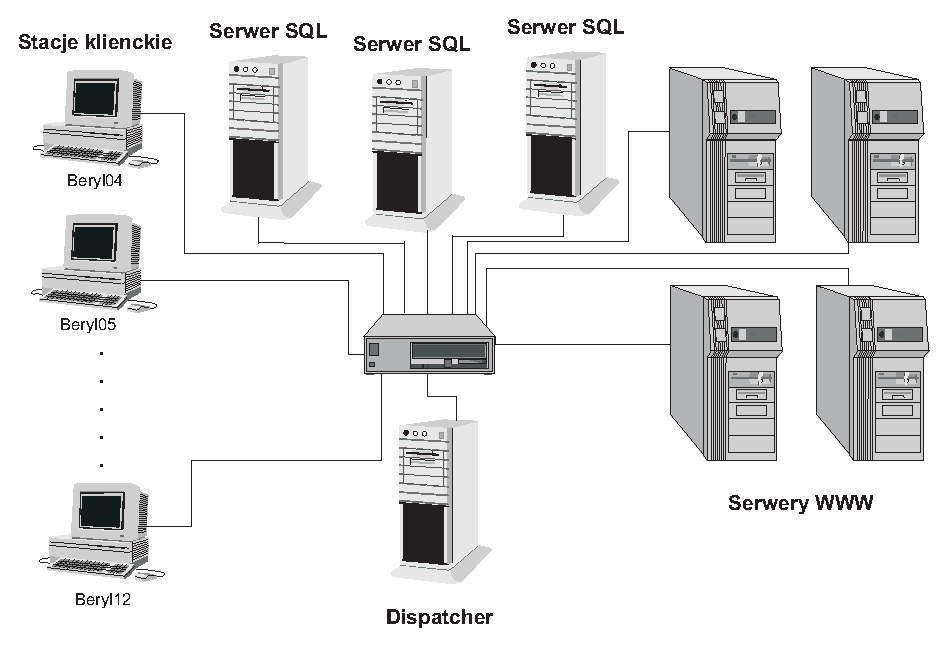
\includegraphics[width=14cm]{./rysunki/komputerki.eps}
\caption{Architektura segmentu sieci testowej.}
\label{architektura}
\end{figure}
Każdy komputer wyposażony był w procesor Intel 
Celeron 300 MHz, 96 MB pamięci SDRAM, dysk twardy o pojemności 3 GB oraz kartę sieciową 3COM EtherLink XL (10/100 Mbps). 
Płyta główna każdego komputera zbudowana była w oparciu o chipset Intel 430 LX. Komputery te posiadały adresy IP z zakresu 
156.17.130.69 -- 156.17.130.79 i nazwy odpowiednio Beryl04 -- Beryl12. Na komputerach tych zainstalowane było oprogramowanie
Astra LoadRunner firmy Mercury Interactive. Komputery o identycznej architekturze stanowiły serwery baz danych: beryl01 (IP = .66), beryl02 (IP = .67), beryl03 (IP = .68).
Zainstalowano na nich MS SQL server w wersji 7.0 (wersja 120 dniowa) wraz z bazą testową.

Poza wyżej wymienionymi komputerami PC podłączony były badany klaster serwerów WWW. Sprzętową platformą serwerów były 
komputery IBM RS 6000 43P Model 260 pracujące pod kontrolą systemu operacyjnego AIX 4.3.3. Każdy z tych komputerów posiadał 
256 MB pamięci RAM, dysk twardy UW SCSI o pojemności 4.3 GB oraz zintegrowaną kartę sieciową IBM 10/100 Mbps. ,,Sercem'' tej 
serii komputerów RS 6000 jest procesor RISC PowerPC Power3 taktowany częstotliwością 200 Mhz. Trzy z wykorzystywanych maszyn 
posiadały jeden taki procesor a dwa wyposażone były w dwa procesory połączone w architekturze SMP. Na każdym z badanych 
serwerów zainstalowane było oprogramowanie serwera WWW Apache for AIX. Poszczególne komputery RS 6000 posiadały adresy IP z 
zakresu 156.17.130.45 -- 156.17.130.49 i nazwy odpowiednio akwamaryn (RS/6000 dwuprocesorowy), szafir (dwuprocesorowy), 
opal01 -- opal03 (jednoprocesorowe). Jedna maszyna dwuprocesorowa (szafir) posłużyła do 
rozpropagowania obciążenia (dispatcher+CBR i WTE), druga posłużyła do obsługi żądań o statyczne
pliki HTML, zaś pozostałe maszyny obsługiwały dynamicznie generowane (poprzez skrypty PHP) strony,
w ten sposób, że każdy z opali pobierał dane z bazy danych poszczególnych beryli (opal01--beryl01,
 opal02--beryl02 i opal03--beryl03).

Wszystkie komputery były połączone ze 100Mbps switchem OmniS/R-5 firmy Alcatel. Również wyjście na Swiat było realizowane z
tą szybkością. 

Konstrukcja zarządzanego, wielokomputerowego systemu WWW była bardzo złożona. Składała się z 
następujących elementów:
\begin{enumerate}
\item Instalacja i konfiguracja switcha OmniSwitch/Router firmy Alcatel;
\item Instalacja i konfiguracja dispatchera z modułem CBR. W skład tej części weszły: 
\begin{itemize}
\item instalacja systemu AIX w wersji 4.3.3 oraz jego update do wersji 4.3.3.0.8 (niezbędne pliki
zostały ściągnięte z odpowiedniej strony firmy IBM;
\item instalacja wirtualnej maszyny (VM) Javy w wersji 1.3.0;
\item instalacja oprogramowania IBM WebSphere Edge Server 1.0.3  wraz z 60--dniową licencją;
\item skonfigurowanie WTE jako \emph{reverse proxy } o adresie URL: www1.ists.pwr.wroc.pl, który
przekierowywał adresy URL do serwerów: opal01, opal02, opal03 i akwamaryn, w ten sposób, aby
żądania o statyczne pliki HTML zostały skierowane do serwera akwamaryn, zaś żądania o dynamicznie
generowane strony z rozszerzeniami: .PHP, .PHP3 i PHP4 zostały rozpropagowane na pozostałe
trzy maszyny;
\end{itemize}
\item Instalacja i konfiguracja oprogramowania dodatkowego na poszczególne serwery WWW i 
dispatchera tzn. HTTP Server Apache w wersji 1.3.19, kompilator C i C++ w postaci gcc w wersji
2.95.3 oraz języka skryptowego PHP w wersji 4.0.6;
\item Instalacja i konfiguracja Windows NT 4.0 Server wraz z Service Pack 6.0 na dwunastu
laboratoryjnych komputerach PC;
\item Instalacja i konfiguracja Microsoft SQL Serwera w wersji 7.0 na serwerach baz danych oraz
instalacja bazy testowej;
\item Instalacja oprogramowania do testów na pozostałych komputerach; przygotowanie testu;
\item przygotowanie witryny WWW do testów;
\end{enumerate}

\subsection{Algorytmy i metody}
Poniżej znajdują się opisane trzy powstałe modele. W każdym z nich program komputer (RS/6000) wraz z zainstalowanym programem 
IBM SecureWay Network Dispatcher stanowi układ rozdysponujący żądaniami. 

\subsubsection{Information less -- moduł dispatcher + Round Robin}

Sam Dispatcher nie ma możliwości pracy w statycznym algorytmie Round Robin, jednakże (jak napisano powyżej, w charakterystyce 
oprogramowania) można posługiwać się modułem Dispatcher z wyłączonym modułem Zarządcy oraz z ogórnie nadanymi wagami. W tym
przypadku, pomimo niehomogenicznego środowiska nadano wszystkim elementom klastra WWW wagi równe jeden. W tej sytuacji komputer
z zainstalowanym dispatcherem równomiernie (bez jakiejkolwiek analizy) propagował żądania do poszczególnych komputerów.

W tym przypadku dostęp do bazy danych mógł być realizowany z dowolnego komputera (serwera WWW).

\subsubsection{Server info aware -- moduł dispatcher + Weighted Round Robin}

W porównaniu do poprzedniego przypadku w tym użyto Dispatchera z uruchomionym modułem zarządcy. Wtedy też realizowany był
algorytm Ważony Round--Robin. Wagi nadawane były dynamicznie tzn. w zależności od obciążenia poszczególnych komputerów -- 
serwerów WWW. 

W tym jak i w powyższym przypadku dostęp do bazy mógł być również realizowany z dolwolnego z serwerów WWW.

\subsubsection{Client info aware -- moduł CBR + WTE}

Był to najbardziej złożony przypadek. Każdy pakiet był analizowany pod względem typu zawartości oraz pod względem jego 
obecności w keszu komponentu WTE. CBR został tak skonfigurowany aby rozpoznawać URL z zawartym w nim wyrazem .php 
(identyfikującym plik HTML z zawartym kodem PHP dostępu do bazy). Pozwoliło to na rozdzdział zapytań na żądania o pliki
statyczne (te były rozsyłane go trzech jednoprocesorowych maszyn RS/6000), zaś te żądania o pliki, których część była
generowana dynamicznie były przekazywane na dwuprocesorowy serwer, który komunikował sie (tylko on) z serwerem baz danych.
Taka konfiguracja pozwoliła rozdysponować zarówno obciążenie jak i typ połączeń.

\subsection{Metodologia testowania}

Celem testowania powstałego systemu do zarządzania wielokomputerowym serwerem WWW
jest zbadanie wydolności takiego systemu -- tzn. jego wydajności w sytuacji
maksymalnego obciążenia, czyli także możliwości odpowiedzi na klienckie 
żądanie w takiej sytuacji. Zamierzeniem testowania jest odpowiedź na 
pytanie jak obciążenie jest równoważone pomiędzy poszczególnymi częściami
składowymi systemu, w zależności od algorytmu dysypacji obciążenia
(Round--Robin, Weighted Round--Robin oraz rozproszenie oparte na CBR), oraz
jaki dany algorytm ma wpływ na LB.

Testowanie zaprojektowanego rozproszonego serwera WWW polegało na pomiarze
wydajności tak wejściowej jak i wyjściowej całego systemu jak i poszczegolnych
jego składowych (poszczególnych serwerów WWW, serwera baz danych i dispatchera).

Celem testowania było zbadanie maksymalnej wydajności systemu. Wydajność systemu można badać na kilka sposobów:
\begin{itemize}
\item ilość zapytań w czasie,
\item ilość danych przesłanych w czasie.
\end{itemize}

Na wynik wpływ ma informacja w jaki sposób rozłożone były zapytania oraz czy sesje kończyły się prawidłowo. Założono trzy 
możliwości odpowiedzi systemu:
\begin{itemize}
\item w czasie do 3 s.,
\item w czasie 5 s.,
\item odpowiedz powyżej 8 s.
\end{itemize}

Za sesję prawidłowo zakończoną uznno taką, podczas której dwie kolejne odpowiedzi na pytania nie przekroczyły 8 s.

Założono następujące ścieżki poruszania się po serwisie \cite{savoia3}:
\begin{itemize}
\item \emph{Home ---> Exit} (Home -- strona domowa);
\item \emph{Home ---> First Level ---> Exit} (First Level -- np. informacja o produkcie);
\item \emph{Home ---> First Level ---> Object ---> Exit} (Object -- np. zakup).
\end{itemize}
Przy założeniu, że ruch na ,,typowej'' witrynie \cite{savoia1,savoia2,savoia3} wygląda w następujący sposób:
\begin{itemize}
\item \emph{Home} -- 58 \%;
\item \emph{First Level} -- 31 \%;
\item \emph{Object} -- 11 \%;
\end{itemize}

Na bazie powyższych danych należy zbudować skrypty generujące zapytania.

\subsubsection{Analiza wyników}

Aby prawidłowo odpowiedzieć na pytanie związane z wydajnością i dostępnością systemu należy podać, 
przy jakiej ilości użytkowników system jest w stanie prawidłowo odpowiadać czyli
przy \emph{x} użytkowników (otwartych sesji) system odpowiada (pomiary zostają wykonanywane w określonych przedziałach 
czasowych):
\begin{itemize}
\item \% w czasie do 3 s.
\item \% w czasie do 5 s.
\item \% powyżej 8 s.
\end{itemize}

Jeżeli podczas sesji dwie następujące po sobie odpowiedzi przekroczyły 8s. -- oznacza to, że ich sesje zostały zerwane.
System nie może być obciążony w większym stopniu niż aktualny aby wszystkie napływające do niego sesje zostały 
prawidłowo obsłużone.

Tak zaplanowane testy należy wykonać podczas pracy Dispatcher--a z różnymi algorytmami: Round Robin, Multi Class Round Robin,
Weighted Round Robin. Wyniki powyższych testów pozwalają sprawdzić, jak zachowuje się system w przypadku chwilowego dużego 
obciążenia. 

Kolejnym elementem testów byłoby zasymulowanie normalnych warunków pracy systemu na granicy 80 \% wydajności. Podczas takiej 
pracy należałoby wygenerować obciążenie znacznie przewyższające możliwości systemu. Obciążenie to powinno trwać 3s, 5s, więcej 
niż 8s. Pozwoli to sprawdzić jak system reaguje i jak szybko jest w stanie się ustabilizować doprowadzając do równego 
rozłożenia obciążenia na poszczególne serwery. 
\section{Wyniki wstępnych eksperymentów}

Na skutek poważnych problemów, tak sprzętowych jak i programowych autor pracy nie zdołał 
zrealizować wszystich zaplanowanych zadań. Poniżej wymieniono kolejne elementy budowy systemu do zarządzania wielokomputerowym
serwerem WWW oraz stopień ich realizacji. 
\begin{enumerate}
\item przygotowano środowisko serwerów front--endowych oraz dispatchera:
\begin{itemize}
\item uruchomiono oraz zainstalowano system operacyjny AIX 4.3.3 na komputerach IBM RS/6000, ktore miały stanowić serwer
dispatchera, oraz cztery serwery WWW; na tych również maszynach wykonano niezbędny update do wersji 4.3.3.0.8;
\item zainstalowano menadżer pakietów RPM, kompilator gcc 2.95.3, Apache 1.3.19 oraz język skryptowy PHP 4.0.6 (za jego pomocą
należało stworzyć interface pomiędzy serwerem WWW a serwerem baz danych) -- jako moduł ładowalny do serwera Apache;
\item skonfigurowano każdy z serwerów WWW wraz z modułem ładowalnym PHP;
\item zainstalowano i skonfigurowano IBM WebSphere Edge Server jako \emph{reverse proxy} wraz z modułem CBR odpowiedzialnym
za specyficzne, oparte na regułach przekierowywanie żądań; podczas instalacji napotkano jednakże na dwa poważne problemy, które
uniemożliwiały instalację, a tym samym działanie pakietu: moduł dispatcher nie uruchamiał się zgłaszając brak pliku licencji,
zaś WTE nie uruchamiał się z powodu niekompatybilności z główną biblioteką systemową (libc.a) (na obie sytuacje nie znaleziono
pomocy w żadnej posiadanej literaturze); skorzystano z \emph{supportu} firmy IBM; w pierwszym przypadku -- otrzymano poprawny
plik licencyjny, zaś w drugim rozwiązaniem okazało się przełączenie urządzeń I/O w tryb asynchroniczny; po wykonaniu obu zadań
oraz skonfigurowaniu modułów -- dispatcher + WTE działało poprawnie;
\end{itemize}
\item przygotowano środowisko serwerów back-endowych (baz danych):
\begin{itemize}
\item zainstalowano na trzech komputerach PC system operacyjny Windows NT 4.0 Server wraz z serwerem baz danych Microsoft
SQL Server 7.0 (wersja 120--dniowa), następnie skonfigurowano te maszyny;
\item zainstalowano bazę testową na serwerach;
\end{itemize}
\item system testowy Astra LoadRunner; niestety nie udało się uzyskać tego oprogramowania testowego z powodu braku wersji 
testowej (komercyjna kosztuje około 13000\$); uzyskano jednakże program Astra LoadTest o zbliżonej funkcjonalności (wersja 
testowa na dzisięciu wirtualnych użytkowników działająca bez ograniczeń 7 dni); został zainstalowany i sprawdzony w kierunku
wymagań tej pracy; wykonano za jego pomocą wstępny, przykładowy test, opis i wyniki znajdują się 
w Dodatku;
\end{enumerate}

Po poprawnym wykonaniu wyżej wymienionych czynności autor pracy stanął przed problemem pobierania danych z serwerów baz danych
przez serwery WWW. Pakiet RPM języka PHP zawierał binarny moduł ładowalny do Apache skompilowany bez wsparcia w komunikacji
z bazami danych (poza samym modułem ładowalnym istnieją jeszcze moduły odpowiadające komunikacji z poszczególnymi serwerami
baz danych). W związku z tym, że PHP jest językiem, który jest dostępny w źródłach (na licencji GPL) próbowano poprzez 
kompilację i odpowiednią konfigurację włączyć go do Apache. MS SQL Server jest serwerem baz danych opartym na motorze firmy 
Sybase, dlatego aby nawiązać komunikację z serwera WWW do serwera bazy danych MS SQL poprzez PHP należało przygotować 
(przekompilować) odpowiednie moduły (klienty) PHP w formie modułów ładowalnych. Niestety z powodu braku odpowiedniego API
nie udało się tego zadania zrealizować (aby móc stworzyć klienty PHP do baz danych -- należy kompilować PHP wraz z API
odpowiedniego serwera bazy danych).

Próbowano także skorzystać z odpowiednich sterowników ODBC firmy OpenLink\footnote{http://www.openlinksw.com}. Poza 
ograniczeniami w korzystaniu z tego oprogramowania (możliwość pracy tylko dwóch jednoczesnych użytkowników podczas sesji) nie
udało się przekompilować PHP (występowały błędy podczas kompilacji). Podczas poszukiwania rozwiązania w Internecie, skorzystano
również z możliwości Usenetu (listy dyskusyjne).

Powyższego problemu nie udało się również rozwiązać analizując zmianę języka oprogramowania: PERL (kolejny znakomity język 
skryptowy umożliwiający generowanie stron dynamicznych) -- ma zbliżone wymagania jeśli chodzi o klientów baz danych, ASP (nie 
istnieje na maszyny Unixowe), C, C++ lub Java (duże kłopoty implementacyjne, spora pracochłonność).

W związku z brakiem możliwości scalenia sewerów WWW z serwerami baz danych nie udało się przetestować w pełni działającego
systemu do zarządzania wielokomputerowym serwisem WWW.
